\documentclass{revtex4-2}
\usepackage{amsmath,hyperref,graphicx}
\begin{document}
\title{URG analysis of the extended Kondo model with interactions in various angular momentum channels}
\author{Abhirup Mukherjee, Siddhartha Lal}
\maketitle
\section{Hamiltonian}
We consider an impurity spin \(\vec S_d\) interacting with a two-dimensional tight-binding conduction bath through a general interaction of the form
\begin{equation}\begin{aligned}
		\sum_{{\bf k}_1, {\bf k}_2, \sigma_1, \sigma_2} J_{{\bf k}_1, {\bf k}_2} \vec{S}_d\cdot\frac{1}{2}\vec{\tau}_{\sigma_1,\sigma_2} c^\dagger_{{\bf k}_1,\sigma_1}c_{{\bf k}_2,\sigma_2}
\end{aligned}\end{equation}
where \(\vec \tau\) is the vector of sigma matrices and \({\bf k}_1,{\bf k}_2\) are momentum states of the conduction bath. The precise form of \(J_{{\bf k}_1, {\bf k}_2}\) depends on the symmetry of the symmetry of the impurity-bath interaction. We consider the following three cases:

(i)~a d-wave interaction, where the impurity couples with a coherent d-wave combination \(f_\sigma\) of the bath sites closest to it: \(f_\sigma \equiv \frac{1}{2}\left(c^\dagger_{L,\sigma} + c^\dagger_{R,\sigma} - c^\dagger_{U\sigma} - c^\dagger_{D\sigma}\right)\), where \(L,R,U\) and \(D\) indicate electrons at the positions \((x,y)=\left(-a,0\right), \left( a,0 \right) , \left( 0,a \right) \) and \(\left( 0,-a \right) \) respectively, \(a\) being the lattice spacing of the conduction bath lattice. The corresponding interaction (in real space) is of the form \(\vec{S}_d\cdot\sum_{\sigma_1,\sigma_2}\frac{1}{2}\vec{\tau}_{\sigma_1,\sigma_2}f^\dagger_{\sigma_1}f_{\sigma_2}\). When fourier-transformed to momentum space, it gives rise to the momentum-dependent Kondo coupling 
\begin{equation}\begin{aligned}\label{J_dwave}
	J_{{\bf k}_1, {\bf k}_2} = J\prod_{i=1,2}\left[\cos\left( ak_i^x \right) - \cos\left( ak_i^y \right) \right]~.
\end{aligned}\end{equation}
For reference, we define the Fourier transforms as \(c^\dagger_{L(R),\sigma} = \sum_{{\bf k}}c^\dagger_{{\bf k},\sigma}e^{-(+)ik^x a}\), \(c^\dagger_{U(D),\sigma} = \sum_{{\bf k}}c^\dagger_{{\bf k},\sigma}e^{-(+)ik^y a}\).

(ii)~a p-wave interaction, where the impurity couples with the p-wave electron \(p_\sigma \equiv \frac{1}{2}\left(c^\dagger_{L,\sigma} + c^\dagger_{R,\sigma} + c^\dagger_{U\sigma} + c^\dagger_{D\sigma}\right)\). The momentum-dependent Kondo coupling in this case is 
\begin{equation}\begin{aligned}\label{J_pwave}
	J_{{\bf k}_1, {\bf k}_2} = J\prod_{i=1,2}\left[\cos\left( ak_i^x \right) + \cos\left( ak_i^y \right) \right]
\end{aligned}\end{equation}
Since we are considering a 2-dimensional conduction bath in the tight-binding limit, such a Kondo coupling vanishes close to the Fermi surface. As a result, this case is not interesting for our purpose.

(iii)~a p-wave interaction, but without the off-site terms in the bath. This amounts to considering the Kondo interaction term \(J\vec{S}_d\cdot\sum_{\sigma_1,\sigma_2}\frac{1}{2}\vec{\tau}_{\sigma_1,\sigma_2}\frac{1}{4}\sum_{i=L,R,U,D}c^\dagger_{i,\sigma_1}c_{i,\sigma_2}\). The momentum-dependent Kondo coupling in this case is 
\begin{equation}\begin{aligned}\label{J_pwave_nooffsite}
	J_{{\bf k}_1, {\bf k}_2} \equiv \frac{1}{2}J \cos\left[ a\left( k_1^x - k_2^x \right) + x\to y \right]
\end{aligned}\end{equation}
This does not vanish identically on the Fermi surface, and is therefore of potential interest to us.

We also consider correlation terms on the bath sites \(L,R,U\) and \(D\). In momentum space, it is of the general form
\begin{equation}\begin{aligned}
-\frac{1}{2}\sum_{1, 2, 3, 4}\sum_\sigma W_{1,2,3,4}~ c^\dagger_{{\bf k}_1,\sigma}c_{{\bf k}_2,\sigma}\left(c^\dagger_{{\bf k}_3,\sigma}c_{{\bf k}_4,\sigma} - c^\dagger_{{\bf k}_3,\bar\sigma}c_{{\bf k}_4,\bar\sigma}\right) ~,
\end{aligned}\end{equation}
where the form of \(W_{\left\{{\bf k}_i\right\}}\) is again determined by the orbitals participating in the interaction. We ignore the p-wave interaction (for the same reason as above) and consider just the d-wave interaction and a p-wave interaction without off-site terms. These two cases lead to the following Hamiltonian structures:
(i)~a d-wave interaction, of the form \(-\frac{W}{2}\left(f^\dagger_{\uparrow}f_{\uparrow} - f^\dagger_{\downarrow}f_{\downarrow}\right)^2\) in real space, leading to the momentum-dependence
\begin{equation}\begin{aligned}\label{W_dwave}
	W_{1,2,3,4} = W\prod_{i=1,2,3,4}\left[\cos\left( ak_i^x \right) - \cos\left( ak_i^y \right) \right]~.
\end{aligned}\end{equation}
(ii)~a p-wave interaction without off-site terms, \(-\frac{W}{2}\sum_{i=L,R,U,D}\left(c^\dagger_{i,\uparrow}c_{i,\uparrow} - c^\dagger_{i,\downarrow}c_{i,\downarrow}\right)^2\), leading to the following form in momentum space:
\begin{equation}\begin{aligned}\label{W_pwave_nooffsite}
	W_{\left\{{\bf k}_i\right\}} = \frac{1}{4}W\left[\cos\left(a\left(k_1^x - k_2^x + k_3^x - k_4^x\right)\right) + x \to y\right]~.
\end{aligned}\end{equation}

To summarise, the total Hamiltonian we consider is of the form
\begin{equation}\begin{aligned}\label{hamiltonian}
	H = -2t\sum_{kx,k y}\left[\cos(ak_x) + \cos(ak_y)\right] c^\dagger_{{\bf k},\sigma}c_{{\bf k},\sigma} + \sum_{{\bf k}_1, {\bf k}_2, \sigma_1, \sigma_2} J_{{\bf k}_1, {\bf k}_2} \vec{S}_d\cdot\frac{1}{2}\vec{\tau}_{\sigma_1,\sigma_2} c^\dagger_{{\bf k}_1,\sigma_1}c_{{\bf k}_2,\sigma_2} \\
-\frac{1}{2}\sum_{1, 2, 3, 4}\sum_\sigma W_{1,2,3,4}~ c^\dagger_{{\bf k}_1,\sigma}c_{{\bf k}_2,\sigma}\left(c^\dagger_{{\bf k}_3,\sigma}c_{{\bf k}_4,\sigma} - c^\dagger_{{\bf k}_3,\bar\sigma}c_{{\bf k}_4,\bar\sigma}\right)~,
\end{aligned}\end{equation}
where \(J_{\left\{ {\bf k}_i \right\} }\) takes one of the two forms in eqs.~\ref{J_dwave} and \ref{J_pwave_nooffsite}, and \(W_{\left\{{\bf k}_i\right\}}\) can similarly take either of the two forms in eqs.~\ref{W_dwave} and \ref{W_pwave_nooffsite}. 

\section{RG scheme}
At any given step \(j\) of the RG procedure, we decouple the states \(\left\{ {\bf q} \right\} \) on the isoenergetic surface of energy \(\varepsilon_j\). The diagonal Hamiltonian \(H_D\) for this step consists of all terms that do not change the occupancy of the states \(\left\{{\bf q}\right\}\):
\begin{equation}\begin{aligned}
	H_D^{(j)} = \varepsilon_j\sum_{q,\sigma}\tau_{q,\sigma} + \frac{1}{2}\sum_{{\bf q}}J_{{\bf q}, {\bf q}}S_d^z\left(\hat n_{{\bf q}, \uparrow} - \hat n_{{\bf q}, \downarrow}\right) - \frac{1}{2}\sum_{{\bf q}}W_{\bf q}\left(\hat n_{{\bf q}, \uparrow} - \hat n_{{\bf q}, \downarrow}\right)^2~,
\end{aligned}\end{equation}
where \(\tau = \hat n - 1/2\) and \(W_{{\bf q}}\) is a shorthand for \(W_{{\bf q},{\bf q},{\bf q},{\bf q}}\). The three terms, respectively, are the kinetic energy of the momentum states on the isoenergetic shell that we are decoupling, the spin-correlation energy between the impurity spin and the spins formed by these momentum states and, finally, the local correlation energy associated with these states arising from the \(W\) term. The off-diagonal part of the Hamiltonian on the other hand leads to scattering in the states \(\left\{ {\bf q} \right\} \). We now list these terms, classified by the coupling they originate from.

\paragraph{Arising from the Kondo spin-exchange term}
\begin{equation}\begin{aligned}
	T_{K1}^\dagger + T_{K1} &= \sum_{{\bf k}, {\bf q}, \sigma,\sigma^\prime}J_{{\bf k}, {\bf q}} \vec{S}_d\cdot\vec{\tau}_{\sigma,\sigma^\prime}\left[c^\dagger_{{\bf q}\sigma}c_{{\bf k},\sigma^\prime} + \text{h.c.}\right],\\
	T_{K2} &= \sum_{{\bf q}, {\bf q}^\prime, \sigma,\sigma^\prime}J_{{\bf k}, {\bf q}} \vec{S}_d\cdot\vec{\tau}_{\sigma,\sigma^\prime}c^\dagger_{{\bf q}\sigma}c_{{\bf q}^\prime,\sigma^\prime}
\end{aligned}\end{equation}
\paragraph{Arising from spin-preserving scattering within conduction bath}
\begin{equation}\begin{aligned}
	T_{P1}^\dagger + T_{P1} &= -\sum_{{\bf q} \in \varepsilon_j}\sum_{{\bf k}_2, {\bf k}_3, {\bf k}_4 < \varepsilon_j}\sum_{\sigma} \left[W_{{\bf q},{\bf k}_2,{\bf k}_3,{\bf k}_4}c^\dagger_{{\bf q},\sigma}c_{{\bf k}_2,\sigma}c^\dagger_{{\bf k}_3,\sigma}c_{{\bf k}_4,\sigma} + \text{h.c.}\right]\\
	T_{P2}^\dagger + T_{P3} &= -\sum_{{\bf q} \in \varepsilon_j}\sum_{{\bf k}_2 < \varepsilon_j}\sum_{\sigma} W_{{\bf q},{\bf k}_2,{\bf \bar q}, {\bf \bar q}} c^\dagger_{{\bf q},\sigma}c_{{\bf k}_2,\sigma} n_{{\bf \bar q},\sigma} -\sum_{{\bf q} \in \varepsilon_j}\sum_{{\bf k}_1 < \varepsilon_j}\sum_{\sigma} W_{{\bf k}_1,{\bf q},{\bf q},{\bf q}} c^\dagger_{{\bf k}_1,\sigma}c_{{\bf q},\sigma} n_{{\bf q},\sigma}
\end{aligned}\end{equation}
\paragraph{Arising from spin-flip scattering within conduction bath}
\begin{equation}\begin{aligned}
	T_{F1}^\dagger + T_{F1} &= \sum_{{\bf q} \in \varepsilon_j}\sum_{{\bf k}_2, {\bf k}_3, {\bf k}_4 < \varepsilon_j}\sum_{\sigma} \left[W_{{\bf q},{\bf k}_2,{\bf k}_3,{\bf k}_4}c^\dagger_{{\bf q},\sigma}c_{{\bf k}_2,\sigma}c^\dagger_{{\bf k}_3,\bar\sigma}c_{{\bf k}_4,\bar\sigma} + \text{h.c.}\right]\\
	T_{F2} &= \sum_{{\bf q}, {\bf q}^\prime \in \varepsilon_j}\sum_{{\bf k}_2, {\bf k}_3 < \varepsilon_j}\sum_{\sigma}W_{{\bf q},{\bf q}^\prime,{\bf k}_2,{\bf k}_3} c^\dagger_{{\bf q},\sigma}c_{{\bf q}^\prime,\sigma}c^\dagger_{{\bf k}_2,\bar\sigma}c_{{\bf k}_3,\bar\sigma}\\
	T_{F3} &= \sum_{{\bf q}, {\bf q}^\prime \in \varepsilon_j}\sum_{{\bf k}_2, {\bf k}_3 < \varepsilon_j}\sum_{\sigma} W_{{\bf q},{\bf k}_2,{\bf k}_3,{\bf q}^\prime} c^\dagger_{{\bf q},\sigma}c_{{\bf k}_2,\sigma}c^\dagger_{{\bf k}_3,\bar\sigma}c_{{\bf q}^\prime,\bar\sigma} \\
	T_{F4}^\dagger + T_{F4} &= \sum_{{\bf q}, {\bf q}^\prime, {\bf q}^{\prime\prime} \in \varepsilon_j}\sum_{{\bf k}_1 < \varepsilon_j}\sum_{\sigma} \left[W_{{\bf q},{\bf q}^\prime,{\bf q}^{\prime\prime}, {\bf k}_1}c^\dagger_{{\bf q},\sigma}c_{{\bf q}^\prime,\sigma}c^\dagger_{{\bf q}^{\prime\prime},\bar\sigma}c_{{\bf k}_1,\bar\sigma} + \text{h.c.}\right]
\end{aligned}\end{equation}
In most of the terms, the factor of \(1/2\) in front has been cancelled out by a factor of 2 coming from the multiple possibilities of arranging the momentum labels.

The renormalisation of the Hamiltonian is constructed from the general expression
\begin{equation}\begin{aligned}
	\Delta H^{(j)} = H_X \frac{1}{\omega- H_D} H_X~.
\end{aligned}\end{equation}

The states on the isoenergetic shell \(\pm|\varepsilon_j|\) come in particle-hole pairs \(\left( {\bf q}, {\bf \bar q} \right) \) with energies of opposite signs (relative to the Fermi energy). If \({\bf q}\) is defined as the hole state (unoccupied in the absence of quantum fluctuations), it will have positive energy, while the particle state \({\bf \bar q}\) will be of negative energy and hence below the Fermi surface. To be more specific, given a state \({\bf q}\) with energy \(\pm|\varepsilon_j|\), we define its particle-hole transformed counterpart as the state \({\bf \bar q} = \boldsymbol{\pi} + {\bf q}\), having energy \(\mp|\varepsilon_j|\) and residing in the opposite quadrant of the Brillouin zone. Given this definition, we have the important property that
\begin{equation}\begin{aligned}\label{particleHoleRelation}
	J_{{\bf k}, {\bf \bar q}} &= -J_{{\bf k}, {\bf q}},\\
	W_{\left\{{\bf k}\right\}, {\bf \bar q}} &= -W_{\left\{{\bf k}\right\}, {\bf q}}~.
\end{aligned}\end{equation}

\begin{figure}[htpb]
	\centering
	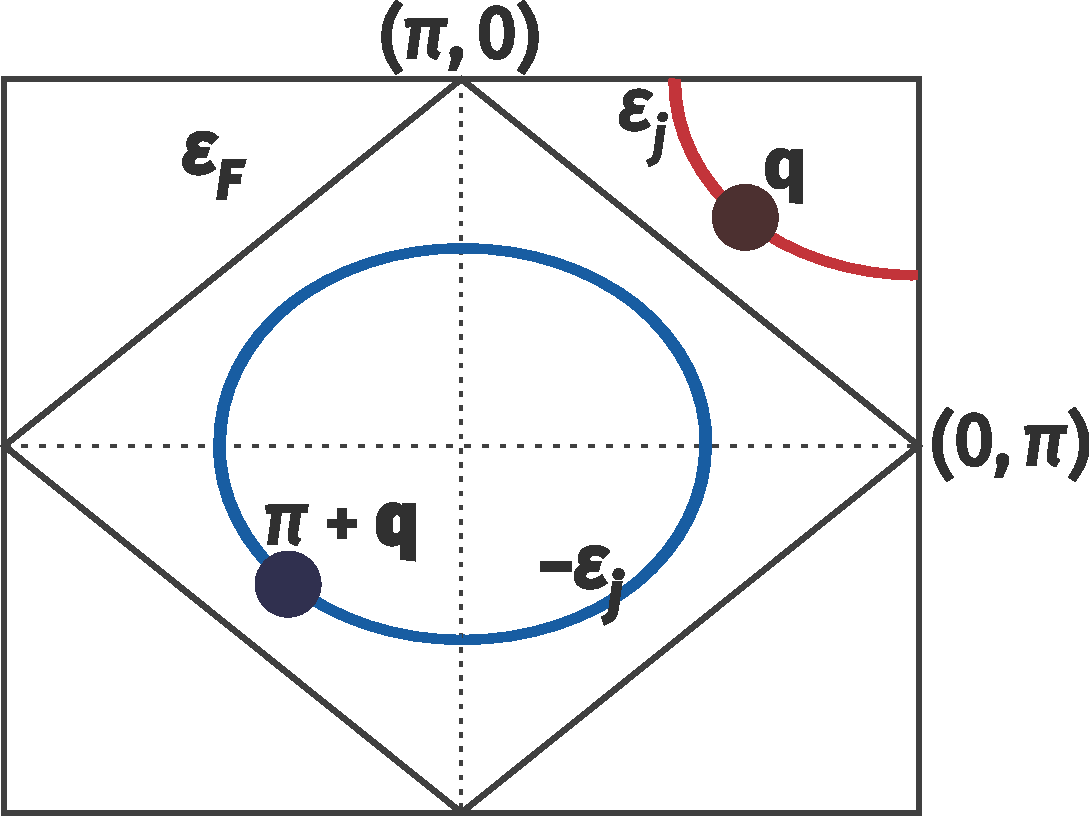
\includegraphics[width=0.48\textwidth]{particleHoleRelation.pdf}
	\caption{Particle and hole states.}
	\label{fig:particleHoleRelation-pdf}
\end{figure}

\section{Renormalisation of the bath correlation term \(W\)}
The bath correlation term \(W\) can undergo renormalisation only via scattering processes arising from itself. Irrespective of whether the state \({\bf q}\) being decoupled is in a particle or hole configuration in the initial many-body state, the propagator \(G = 1/(\omega - H_D)\) of the intermediate excited state is uniform, and equal to 
\begin{equation}\begin{aligned}\label{propagatorW}
	G_W = 1/\left(\omega - |\varepsilon_j|/2 + W_{\bf q}/2)\right)~,
\end{aligned}\end{equation}
where \(W_{\bf q}\) is the same whether \({\bf q}\) is above or below the Fermi surface. The \(|\varepsilon_j|/2\) in \(H_D\) arises from the excited nature of the state after the initial scattering process.

\subsection{Scattering arising purely from spin-preserving processes}
In this subsection, we calculate the renormalisation to \(W\) arising from the terms \(T_{P1}\), \(T_{P2}\) and \(T_{P3}\). The first term is
\begin{equation}\begin{aligned}
	T_{P1}^\dagger G_W T_{P3} &= \sum_\sigma\sum_{{\bf k}_1, {\bf k}_2, {\bf k}_3, {\bf k}_4} \sum_{\bf q} W_{{\bf q},{\bf k}_2,{\bf k}_3,{\bf k}_4}c^\dagger_{{\bf q},\sigma}c_{{\bf k}_2,\sigma}c^\dagger_{{\bf k}_3,\sigma}c_{{\bf k}_4,\sigma} G_W W_{{\bf k}_1,{\bf q},{\bf q},{\bf q}} c^\dagger_{{\bf k}_1,\sigma}c_{{\bf q},\sigma} n_{{\bf q},\sigma}\\
							  &= -\sum_\sigma\sum_{{\bf k}_1, {\bf k}_2, {\bf k}_3, {\bf k}_4} c^\dagger_{{\bf k}_1,\sigma} c_{{\bf k}_2,\sigma}c^\dagger_{{\bf k}_3,\sigma}c_{{\bf k}_4,\sigma} \sum_{\bf q \in \text{PS}} W_{{\bf q},{\bf k}_2,{\bf k}_3,{\bf k}_4} G_W W_{{\bf k}_1,{\bf q},{\bf q},{\bf q}}~.
\end{aligned}\end{equation}
The operators acting on the states being decoupled contract to form a number operator \(n_{{\bf q},\sigma}\) which projects the sum over \({\bf q}\) into the states that are initial occupied (particle sector, PS). 

The second such contribution is obtained by flipping the sequence of scattering processes:
\begin{equation}\begin{aligned}
	T_{P3} G_W T_{P1}^\dagger &= \sum_\sigma\sum_{{\bf k}_1, {\bf k}_2, {\bf k}_3, {\bf k}_4} \sum_{\bf q} W_{{\bf k}_1,{\bf q},{\bf q},{\bf q}} c^\dagger_{{\bf k}_1,\sigma}c_{{\bf q},\sigma} n_{{\bf q},\sigma} G_W W_{{\bf q},{\bf k}_2,{\bf k}_3,{\bf k}_4}c^\dagger_{{\bf q},\sigma}c_{{\bf k}_2,\sigma}c^\dagger_{{\bf k}_3,\sigma}c_{{\bf k}_4,\sigma} \\
							  &= \sum_\sigma\sum_{{\bf k}_1, {\bf k}_2, {\bf k}_3, {\bf k}_4} c^\dagger_{{\bf k}_1,\sigma} c_{{\bf k}_2,\sigma}c^\dagger_{{\bf k}_3,\sigma}c_{{\bf k}_4,\sigma} \sum_{\bf q \in \text{HS}} W_{{\bf q},{\bf k}_2,{\bf k}_3,{\bf k}_4} G_W W_{{\bf k}_1,{\bf q},{\bf q},{\bf q}}~.
\end{aligned}\end{equation}
By virtue of eq.~\ref{particleHoleRelation}, the product of couplings \(W_{{\bf q},{\bf k}_2,{\bf k}_3,{\bf k}_4} G_W W_{{\bf k}_1,{\bf q},{\bf q},{\bf q}}\) is the same irrespective of whether \({\bf q}\) belongs to the particle or hole sector. The two contributions therefore cancel each other. Moreover, the remaining contributions \(T_{P3}^\dagger G_W T_{P1}\) and \(T_{P1}G_W T_{P2}^\dagger\) are effectively hermitian conjugates of the two contributions considered above, and therefore also cancel each other.

\subsection{Scattering arising from spin-flip processes}
We now come to the processes that involve spin-flips. Considering \(T_{F1}\) and \(T_{F4}\) first, we get
\begin{equation}\begin{aligned}
	T_{F1}^\dagger G_W T_{F4} &= \sum_\sigma\sum_{{\bf k}_1, {\bf k}_2, {\bf k}_3, {\bf k}_4} \sum_{\bf q} W_{{\bf q},{\bf k}_2,{\bf k}_3,{\bf k}_4}c^\dagger_{{\bf q},\sigma}c_{{\bf k}_2,\sigma}c^\dagger_{{\bf k}_3,\bar\sigma}c_{{\bf k}_4,\bar\sigma} G_W W_{{\bf k}_1, {\bf q}, {\bf q}, {\bf q}}  c^\dagger_{{\bf k}_1\sigma} c_{{\bf q}\sigma} n_{{\bf q} \bar \sigma} \\
							  &= -\sum_{1,2,3,4}\sum_\sigma c^\dagger_{{\bf k}_1\sigma} c_{{\bf k}_2\sigma} c^\dagger_{{\bf k}_3\bar\sigma} c_{{\bf k}_4\bar \sigma} \sum_{\bf q \in \text{PS}} W_{{\bf q}, {\bf k}_2, {\bf k}_4, {\bf k}_4} G_W W_{{\bf k}_1, {\bf q}, {\bf q}, {\bf q}}~,\\
	T_{F4} G_W T_{F1}^\dagger &= \sum_\sigma\sum_{{\bf k}_1, {\bf k}_2, {\bf k}_3, {\bf k}_4} \sum_{\bf q}W_{{\bf k}_1, {\bf q}, {\bf q}, {\bf q}}  c^\dagger_{{\bf k}_1\sigma} c_{{\bf q}\sigma} n_{{\bf q} \bar \sigma} G_W W_{{\bf q},{\bf k}_2,{\bf k}_3,{\bf k}_4}c^\dagger_{{\bf q},\sigma}c_{{\bf k}_2,\sigma}c^\dagger_{{\bf k}_3,\bar\sigma}c_{{\bf k}_4,\bar\sigma}  \\
							  &= \sum_{1,2,3,4}\sum_\sigma c^\dagger_{{\bf k}_1\sigma} c_{{\bf k}_2\sigma} c^\dagger_{{\bf k}_3\bar\sigma} c_{{\bf k}_4\bar \sigma} \sum_{\bf q \in \text{HS}} W_{{\bf q}, {\bf k}_2, {\bf k}_4, {\bf k}_4} G_W W_{{\bf k}_1, {\bf q}, {\bf q}, {\bf q}}~.
\end{aligned}\end{equation}
By the same arguments as in the previous subsection, these terms cancel each other out. Their hermitian conjugate contributions \(T_{F1} G_W T_{F4}^\dagger\) and \(T_{F4}^\dagger G_W T_{F1}\) also cancel out. The other two terms are \(T_{F2}\) and \(T_{F3}\), and their contributions also cancel out for the same reason:
\begin{equation}\begin{aligned}
	T_{F2} G_W T_{F2} &= \sum_\sigma\sum_{{\bf k}_1, {\bf k}_2, {\bf k}_3, {\bf k}_4} \sum_{\bf q}W_{{\bf q},{\bf \bar q},{\bf k}_3,{\bf k}_4} c^\dagger_{{\bf q},\sigma}c_{{\bf \bar q},\sigma}c^\dagger_{{\bf k}_3,\bar\sigma}c_{{\bf k}_4,\bar\sigma} G_W W_{{\bf \bar q},{\bf q},{\bf k}_1,{\bf k}_2} c^\dagger_{{\bf \bar q},\sigma}c_{{\bf q},\sigma}c^\dagger_{{\bf k}_1,\bar\sigma}c_{{\bf k}_2,\bar\sigma} \\
							  &= \sum_{1,2,3,4}\sum_\sigma c^\dagger_{{\bf k}_1\sigma} c_{{\bf k}_2\sigma} c^\dagger_{{\bf k}_3\bar\sigma} c_{{\bf k}_4\bar \sigma} \sum_{\bf q \in \text{PS}} W_{{\bf q},{\bf \bar q},{\bf k}_3,{\bf k}_4} G_W W_{{\bf \bar q},{\bf q},{\bf k}_1,{\bf k}_2}~,\\
	T_{F3} G_W T_{F3} &= \sum_\sigma\sum_{{\bf k}_1, {\bf k}_2, {\bf k}_3, {\bf k}_4} \sum_{\bf q} W_{{\bf q},{\bf k}_2,{\bf k}_3,{\bf \bar q}} c^\dagger_{{\bf q},\sigma}c_{{\bf k}_2,\sigma}c^\dagger_{{\bf k}_3,\bar\sigma}c_{{\bf \bar q},\bar\sigma} G_W W_{{\bf \bar q},{\bf k}_4,{\bf k}_1,{\bf q}} c^\dagger_{{\bf \bar q},\bar\sigma} c_{{\bf k}_4,\bar\sigma} c^\dagger_{{\bf k}_1,\sigma} c_{{\bf q},\sigma} \\
							  &= -\sum_{1,2,3,4}\sum_\sigma c^\dagger_{{\bf k}_1\sigma} c_{{\bf k}_2\sigma} c^\dagger_{{\bf k}_3\bar\sigma} c_{{\bf k}_4\bar \sigma} \sum_{\bf q \in \text{PS}} W_{{\bf q},{\bf k}_2,{\bf k}_3,{\bf \bar q}} G_W W_{{\bf \bar q},{\bf k}_4,{\bf k}_1,{\bf q}}~,
\end{aligned}\end{equation}

\subsection{Scattering involving both spin-flip and spin-preserving processes}
These processes involve the combination of terms like \(T_{P1}\) with \(T_{F4}\), and \(T_{P2}\) with \(T_{F1}\). These again cancel each other out for the same reasons as outline above.

\subsection{Net renormalisation for the bath correlation term}
Since all the contributions cancel out in pairs, the bath correlation term \(W\) is {\it marginal}.

\section{Renormalisation of the Kondo scattering term {\it J}}
\subsection{Impurity-mediated spin-flip scattering purely through Kondo-like processes}
We first consider the renormalisation to the \(S_d^z\) term, arising purely from the Kondo terms:
\begin{equation}\begin{aligned}
	\sum_{\sigma=\pm}T_{1,\sigma\bar\sigma}^\dagger G T_{1,\sigma\bar\sigma} = \sum_{\sigma=\pm}\frac{1}{4}\sum_{{\bf k}_2,{\bf q}}J_{{\bf k}_2,{\bf q}} S_d^\sigma c^\dagger_{{\bf q},\bar\sigma} c_{{\bf k}_2,\sigma} \frac{1}{\omega - H_D}\sum_{{\bf k}_1,{\bf q}}J_{{\bf k}_1,{\bf q}} S_d^{\bar\sigma} c^\dagger_{{\bf k}_1,\sigma} c_{{\bf q},\bar\sigma}~,
\end{aligned}\end{equation}
where \(c_{k,+(-)} \equiv c_{k,\uparrow(\downarrow)}\). The excitation energy for such processes is given by \(H_D = |\varepsilon_j| - J_{{\bf q}}/4 - W_{{\bf q}}/2\), due to the fact that the impurity spin flip and the spin flip of the conduction bath state \({\bf q}\) occurs in an anti-parallel fashion. Substituting this, performing the usual contraction and projection of the state \({\bf q}\) and carrying out the spin manipulation \(S_d^\sigma S_d^{\bar\sigma} = \frac{1}{2} + \sigma S_d^z\) results in the expression
\begin{equation}\begin{aligned}\label{t1t1p}
	\sum_{\sigma=\pm}T_{1,\sigma\bar\sigma}^\dagger G T_{1,\sigma\bar\sigma} &= \sum_{\sigma=\pm}\frac{1}{4}\sum_{{\bf k}_2,{\bf k}_1} \left(\frac{1}{2} + \sigma S_d^z\right) c_{{\bf k}_2,\sigma} c^\dagger_{{\bf k}_1,\sigma}\sum_{{\bf q}}  \hat n_{{\bf q},\bar\sigma} \frac{J_{{\bf k}_2,{\bf q}} J_{{\bf k}_1,{\bf q}}}{\omega - |\varepsilon_j| + J_{{\bf q}}/4 + W_{{\bf q}}/2}\\
										 &= -\frac{1}{2}\sum_{{\bf k}_2,{\bf k}_1} S_d^z \sigma \frac{1}{2}c^\dagger_{{\bf k}_1,\sigma}c_{{\bf k}_2,\sigma} \sum_{{\bf q} \in \text{PS}} \frac{J_{{\bf k}_2,{\bf q}} J_{{\bf k}_1,{\bf q}}}{\omega - |\varepsilon_j| + J_{{\bf q}}/4 + W_{{\bf q}}/2} + \bigg[\text{pot. scatt. terms}\bigg]~.
\end{aligned}\end{equation}
The particle-hole exchanged partner is
\begin{equation}\begin{aligned}\label{t1t1h}
	\sum_{\sigma=\pm}T_{1,\sigma\bar\sigma} G T^\dagger_{1,\sigma\bar\sigma} &= \sum_{\sigma=\pm}\frac{1}{4} \sum_{{\bf k}_1,{\bf q}}J_{{\bf k}_1,{\bf q}} S_d^{\bar\sigma} c^\dagger_{{\bf k}_1,\sigma} c_{{\bf q},\bar\sigma} \frac{1}{\omega - H_D}\sum_{{\bf k}_2,{\bf q}}J_{{\bf k}_2,{\bf q}} S_d^\sigma c^\dagger_{{\bf q},\bar\sigma} c_{{\bf k}_2,\sigma}\\
										 &= \sum_{\sigma=\pm}\frac{1}{4}\sum_{{\bf k}_2,{\bf k}_1} \left(\frac{1}{2} + \bar\sigma S_d^z\right) c^\dagger_{{\bf k}_1,\sigma} c_{{\bf k}_2,\sigma} \sum_{{\bf q}} \left(1 - \hat n_{{\bf q},\bar\sigma}\right) \frac{J_{{\bf k}_2,{\bf q}} J_{{\bf k}_1,{\bf q}}}{\omega - |\varepsilon_j| + J_{{\bf q}}/4 + W_{{\bf q}}/2}\\
										 &= -\frac{1}{2}\sum_{{\bf k}_2,{\bf k}_1, \sigma} S_d^z \sigma \frac{1}{2}c^\dagger_{{\bf k}_1,\sigma}c_{{\bf k},\sigma} \sum_{{\bf q} \in \text{HS}} \frac{J_{{\bf k}_2,{\bf q}} J_{{\bf k}_1,{\bf q}}}{\omega - |\varepsilon_j| + J_{{\bf q}}/4 + W_{{\bf q}}/2} + \bigg[\text{pot. scatt. terms}\bigg]\\
										 &= -\frac{1}{2}\sum_{{\bf k}_2,{\bf k}_1, \sigma} S_d^z \sigma \frac{1}{2}c^\dagger_{{\bf k}_1,\sigma}c_{{\bf k},\sigma} \sum_{{\bf q} \in \text{PS}} \frac{J_{{\bf k}_2,{\bf q}} J_{{\bf k}_1,{\bf q}}}{\omega - |\varepsilon_j| + J_{{\bf q}}/4 + W_{{\bf q}}/2} + \bigg[\text{pot. scatt. terms}\bigg]~.
\end{aligned}\end{equation}
At the last step, we converted the sum over the hole sector into one over the particle sector. As argued elsewhere, transforming from the particle to the hole sector results in the inversion of the sign of the factor \(\left[\cos\left( aq_1^x \right) - \cos\left( aq_1^y \right) \right]\), leaving the product \(J_{{\bf k}_2,{\bf q}} J_{{\bf k}_1,{\bf q}}\) unchanged. The couplings in the denominators involve the product of four such factors, so they also remain unchanged.

\subsection{Scattering processes involving the Kondo interaction as well as the bath interaction}
Next, we consider scattering processes involving \(T_7, T_6\):
\begin{equation}\begin{aligned}\label{t7t6}
	T_{7,z} G T_6 &= \frac{1}{4}\sum_{{\bf k}_1,{\bf k}_2,{\bf q},\sigma}\sigma J_{-{\bf q},{\bf q}}S_d^z c^\dagger_{{\bf q},\sigma} c_{-{\bf q},\sigma} \frac{1}{\omega - H_D} \left(- W_{{\bf q},-{\bf q},{\bf k}_1, {\bf k}_2}\right) \left(2 c^\dagger_{k_1\sigma}c_{k_2\sigma}c^\dagger_{-{\bf q},\sigma}c_{{\bf q},\sigma} - 2 c^\dagger_{k_1\bar\sigma}c_{k_2\bar\sigma}c^\dagger_{-{\bf q},\sigma}c_{{\bf q},\sigma}\right)\\
			      &= -\frac{1}{2}\sum_{{\bf k}_1,{\bf k}_2,{\bf q},\sigma}\sigma S_d^z \left(c^\dagger_{k_1\sigma}c_{k_2\sigma} - c^\dagger_{k_1\bar\sigma}c_{k_2\bar\sigma}\right) \sum_{{\bf q} \in \text{PS}}\frac{J_{-{\bf q},{\bf q}} W_{{\bf q},-{\bf q},{\bf k}_1, {\bf k}_2}}{\omega - |\varepsilon_j| + J_{{\bf q}}/4 + W_{{\bf q}}/2} \\
			      &= -2\sum_{{\bf k}_1,{\bf k}_2,\sigma}\sigma S_d^z \frac{1}{2}c^\dagger_{k_1\sigma}c_{k_2\sigma} \sum_{{\bf q} \in \text{PS}}\frac{J_{-{\bf q},{\bf q}} W_{{\bf q},-{\bf q},{\bf k}_1, {\bf k}_2}}{\omega - |\varepsilon_j| + J_{{\bf q}}/4 + W_{{\bf q}}/2} 
\end{aligned}\end{equation}
Another scattering process is obtained by switching the operators \(T_7\) and \(T_6\):
\begin{equation}\begin{aligned}\label{t6t7}
	T_{6}^\dagger G T_{7,z} &= \frac{1}{4}\sum_{{\bf k}_1,{\bf k}_2,{\bf q},\sigma} \left(- W_{{\bf q},-{\bf q},{\bf k}_1, {\bf k}_2}\right) \left(2 c^\dagger_{k_1\sigma}c_{k_2\sigma}c^\dagger_{-{\bf q},\sigma}c_{{\bf q},\sigma} - 2 c^\dagger_{k_1\bar\sigma}c_{k_2\bar\sigma}c^\dagger_{-{\bf q},\sigma}c_{{\bf q},\sigma}\right) \frac{1}{\omega - H_D} \sigma J_{-{\bf q},{\bf q}}S_d^z c^\dagger_{{\bf q},\sigma} c_{-{\bf q},\sigma}\\
			      &= -\frac{1}{2}\sum_{{\bf k}_1,{\bf k}_2,{\bf q},\sigma}\sigma S_d^z \left(c^\dagger_{k_1\sigma}c_{k_2\sigma} - c^\dagger_{k_1\bar\sigma}c_{k_2\bar\sigma}\right) \sum_{{\bf q} \in \text{HS}}\frac{J_{-{\bf q},{\bf q}} W_{{\bf q},-{\bf q},{\bf k}_1, {\bf k}_2}}{\omega - |\varepsilon_j| + J_{{\bf q}}/4 + W_{{\bf q}}/2} \\
			      &= -2\sum_{{\bf k}_1,{\bf k}_2,\sigma}\sigma S_d^z \frac{1}{2} c^\dagger_{k_1\sigma}c_{k_2\sigma} \sum_{{\bf q} \in \text{HS}}\frac{J_{-{\bf q},{\bf q}} W_{{\bf q},-{\bf q},{\bf k}_1, {\bf k}_2}}{\omega - |\varepsilon_j| + J_{{\bf q}}/4 + W_{{\bf q}}/2} \\
			      &= -2\sum_{{\bf k}_1,{\bf k}_2,\sigma}\sigma S_d^z \frac{1}{2} c^\dagger_{k_1\sigma}c_{k_2\sigma} \sum_{{\bf q} \in \text{PS}}\frac{J_{-{\bf q},{\bf q}} W_{{\bf q},-{\bf q},{\bf k}_1, {\bf k}_2}}{\omega - |\varepsilon_j| + J_{{\bf q}}/4 + W_{{\bf q}}/2} \\
\end{aligned}\end{equation}
At the last step, we again transformed from the particle sector to the hole sector using the arguments mentioned just above.

\subsection{Net renormalisation to the Kondo interaction}
Owing to spin-rotation symmetry of the Kondo interaction, it suffices to calculate the renormalisation for the Ising-like interaction term, since that of the spin-flip terms will be equal to it. Upon adding the Hamltonian renormalisation from the four classes eqs.~\ref{t1t1p}, \ref{t1t1h}, \ref{t7t6} and \ref{t6t7}, the total renormalisation in the Ising part of the Kondo interaction comes out to be
\begin{equation}\begin{aligned}
	\Delta J^{(j)}_{{\bf k}_1, {\bf k}_2} = -\sum_{{\bf q} \in \text{PS}} \frac{J^{(j)}_{{\bf k}_2,{\bf q}} J^{(j)}_{{\bf k}_1,{\bf q}} + 4J^{(j)}_{-{\bf q},{\bf q}} W^{(j)}_{{\bf q},-{\bf q},{\bf k}_1, {\bf k}_2}}{\omega - |\varepsilon_j| + J^{(j)}_{{\bf q}}/4 + W^{(j)}_{{\bf q}}/2}
\end{aligned}\end{equation}


\end{document}
